% Geometric adaptation of the preserved cubic-completion figure.
\begin{figure}[htbp]
\centering
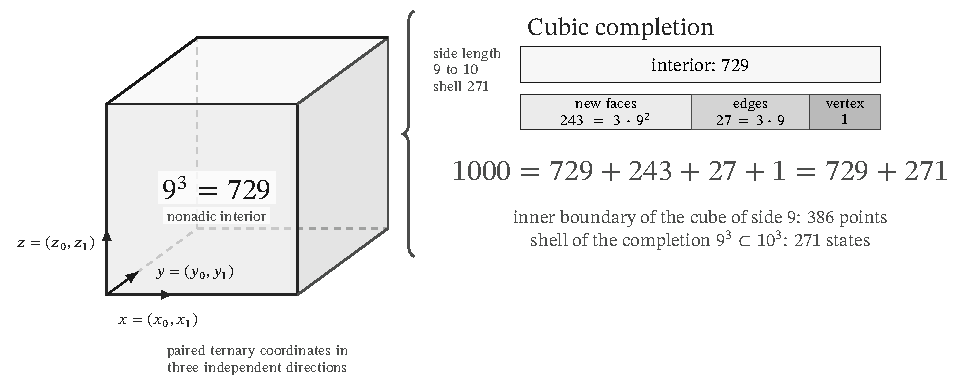
\includegraphics[width=\linewidth]{figures/cubo_emrh_original.pdf}
\caption{Cubic representation of the expansion from nine to ten classes per coordinate. Strata \(S_1,S_2,S_3\) locate the added incidences on faces, edges, and the apex; their cardinalities form the \(271\)-element shell. The \(386\)-element boundary belongs to the initial cube. This geometric perspective complements the partition in Figure~\ref{fig:revision-emrh}; graphical spacing is schematic.}
\label{fig:completacion-cubo-recuperado}
\end{figure}
